\usepackage{graphics} % resizebox
\usepackage{tabu} % awesome table
%\usepackage{etex} % simple math
\usepackage{svg} % for svg images
\usepackage[auto]{contour}
\usepackage{pgfplots} % graphs
\usepackage{algorithm} % for pseudocode
\usepackage{algpseudocode} % for pseudocode
\usepackage{multicol}
\usepackage{adjustbox}
\newcommand{\backupbegin}{
   \newcounter{finalframe}
   \setcounter{finalframe}{\value{framenumber}}
}
\newcommand{\backupend}{
   \setcounter{framenumber}{\value{finalframe}}
}

\pgfplotsset{compat=1.13}
\contourlength{0.15em}

\newcommand\setside[1]{\setbeamertemplate{background}{\includegraphics[width=0.1\paperwidth,height=\paperheight]{img/side#1}}}
\newcount\offset
\offset=7
\newcommand\C[0]{\cellcolor{gray}}
\newcommand\CS[3]{\only<#1-\the\numexpr #2-1 \relax>{\C}\only<#2->{#3}}
\newcommand\CC[2]{\CS{\the\numexpr #1+\offset \relax}{\the\numexpr #1+1+\offset \relax}{#2}}
\newcommand\INIT[1]{\textbf{\only<2>{\cellcolor{yellow}}#1}}
\newcommand\COLOR[3]{\temporal<#2>{#3}{\adjustbox{bgcolor=#1}{\strut $#3$}}{#3}}
\newcommand\CCOLOR[2]{\only<#2>{\cellcolor{#1}}}

\definecolor{red}{HTML}{FF9999}
\definecolor{green}{HTML}{99FF99}
\definecolor{blue}{HTML}{9999FF}

\newcommand\nodea[0]{none}
\newcommand\nodeb[0]{none}
\newcommand\nodec[0]{none}

\background{4}  % choose background {1..5}
\taal{EN}       % EN or NL
\title{Edit distance on GPU clusters using MPI}
\subtitle{Antoine Veenstra}
\date{July 7, 2017}

\begin{document}

\maketitleslide

\setside{1}

%\section{Introduction}
\begin{frame}{Introduction}
\underline{Edit distance} on \underline{GPU} \underline{clusters} using \underline{MPI}

\begin{itemize}
    % what is edit distance
    \item \underline{Edit distance}
    \begin{itemize}
        \item Number of operations
        \item Insertion, deletion, and replacement \pause
        \item Distance between ``\texttt{kitten}'' and ``\texttt{sitting}'':
        \begin{itemize}
                \item Replace the ``\texttt{k}'' with an ``\texttt{s}''.\hfill ``\texttt{kitten}'' $\rightarrow$ ``\texttt{sitten}'' $\qquad\enspace\qquad$
                \item Replace the ``\texttt{e}'' with an ``\texttt{i}''.\hfill ``\texttt{sitten}'' $\rightarrow$ ``\texttt{sittin}'' $\qquad\enspace\qquad$
                \item Insert ``\texttt{g}'' at the end.\hfill ``\texttt{sittin}'' $\rightarrow$ ``\texttt{sitting}'' $\qquad\qquad$ \pause
        \end{itemize}
        \item Used in:
        \begin{itemize}
            \item Computational Biology (DNA and RNA mutations)
            \item Correction of spelling mistakes
            \item Correction of OCR errors
        \end{itemize}
    \end{itemize} \pause
	\item Message Passing Interface (\underline{MPI})
\end{itemize}
\end{frame}

%\setside{1}
%\section{Distribution}
% small matrix
% big matrix
% division in pillars

%\begin{frame}{Edit distance on a computer}
%\begin{table}
%\begin{tabular}{|c|c||c|c|c|c|c|c|} \hline
%           &            & \textbf{k} & \textbf{i} & \textbf{t} & \textbf{t} & \textbf{e} & \textbf{n} \\ %\hline
%           & \textbf{0} & \textbf{1} & \textbf{2} & \textbf{3} & \textbf{4} & \textbf{5} & \textbf{6} \\ %\hline \hline
%\textbf{s} & \textbf{1} &            &            &            &            &            &            \\ \hline
%\textbf{i} & \textbf{2} &            &            &            &            &            &            \\ \hline
%\textbf{t} & \textbf{3} &            &            &            &            &            &            \\ \hline
%\textbf{t} & \textbf{4} &            &            &            &            &            &            \\ \hline
%\textbf{i} & \textbf{5} &            &            &            &            &            &            \\ \hline
%\textbf{n} & \textbf{6} &            &            &            &            &            &            \\ \hline
%\textbf{g} & \textbf{7} &            &            &            &            &            &            \\ \hline
%\end{tabular}
%\end{table}
%\end{frame}

\begin{frame}
% \begin{columns}
% \column{0.1\paperwidth}
% \column{0.4\paperwidth}
%\resizebox{0.99\linewidth}{!}{%
\begin{table}
\begin{tabular}{|c|c||c|c|c|c|c|c|} \hline
           &            & \textbf{k} & \textbf{i} & \textbf{t} & \textbf{t} & \textbf{e} & \textbf{n} \\ \hline
           & \INIT{\CCOLOR{blue}{6-7}0} & \INIT{\CCOLOR{red}{4-7}1} & \INIT{2} & \INIT{3} & \INIT{4} & \INIT{5} & \INIT{6} \\ \hline \hline
\textbf{s} & \INIT{\CCOLOR{green}{5-7}1} & \CS{3}{\offset}{1}  & \CC{2}{2}  & \CC{3}{3} & \CC{4 }{4} & \CC{5 }{5} & \CC{6 }{6}  \\ \hline
\textbf{i} & \INIT{2} & \CC{2}{2}  & \CC{3}{1}  & \CC{4}{2} & \CC{5 }{3} & \CC{6 }{4} & \CC{7 }{5}  \\ \hline
\textbf{t} & \INIT{3} & \CC{3}{3}  & \CC{4}{2}  & \CC{5}{1} & \CC{6 }{2} & \CC{7 }{3} & \CC{8 }{4}  \\ \hline
\textbf{t} & \INIT{4} & \CC{4}{4}  & \CC{5}{3}  & \CC{6}{2} & \CC{7 }{1} & \CC{8 }{2} & \CC{9 }{3}  \\ \hline
\textbf{i} & \INIT{5} & \CC{5}{5}  & \CC{6}{4}  & \CC{7}{3} & \CC{8 }{2} & \CC{9 }{2} & \CC{10}{3}  \\ \hline
\textbf{n} & \INIT{6} & \CC{6}{6}  & \CC{7}{5}  & \CC{8}{4} & \CC{9 }{3} & \CC{10}{3} & \CC{11}{2}  \\ \hline
\textbf{g} & \INIT{7} & \CC{7}{7}  & \CC{8}{6}  & \CC{9}{5} & \CC{10}{4} & \CC{11}{4} & \CC{12}{\cellcolor{green}\textbf{3}} \\ \hline
\end{tabular}
\end{table}%
%}
% \column{0.4\paperwidth}
\newcommand\vi[0]{\text{i}}
\newcommand\vj[0]{\text{j}}
%\resizebox{0.99\linewidth}{!}{%
\begin{equation*}
\begin{split}
\rules
\operatorname{H}{[\vi,\vj]} &= \min
    \begin{cases}
        \COLOR{red}{4-7}{\operatorname{H}{[\vi,\vj-1]} + 1} & \\
        \COLOR{green}{5-7}{\operatorname{H}{[\vi-1,\vj]} + 1} & \\
        \COLOR{blue}{6-7}{\operatorname{H}{[\vi-1,\vj-1]}} &\COLOR{blue}{6-7}{\quad \text{if } s_{a}{[\vi]} = s_{b}[\vj]}\\
        \COLOR{blue}{6-7}{\operatorname{H}{[\vi-1,\vj-1]} + 1} &\COLOR{blue}{6-7}{ \quad \text{if } s_{a}{[\vi]} \neq s_{b}[\vj]}\\
    \end{cases}
\end{split}
\end{equation*}
\end{frame}

\begin{frame}
    \includesvg[height=0.85\paperheight]{bigtable}
\end{frame}
\begin{frame}
    \includesvg[height=0.85\paperheight]{bigtable2}
\end{frame}
\begin{frame}
    \includesvg[height=0.85\paperheight]{bigtable3}
\end{frame}
\begin{frame}
    \includesvg[height=0.85\paperheight]{bigtable4}
\end{frame}
\begin{frame}
    \includesvg[height=0.85\paperheight]{bigtable5}
\end{frame}

\begin{frame}{Implementation}
    \begin{itemize}
    	\item OpenCL
        \item C++
        \item OpenMPI
        \item Permission based verification
        \item Static partitioning
    \end{itemize}
\end{frame}


\begin{frame}{Test results}
    \begin{itemize}
        \item Two nodes:
        \item Maximum tested: $12.0\cdot10^{10}$ cells ($\pm 113$s)
        \item Comparing two chromosomes: $5.5\cdot10^{16}$ cells ($\pm 1.7$y)\pause
    \end{itemize}
	\begin{tabular}{l r r}
		\textbf{Name} & \textbf{Compute Units} & \textbf{Average compute time} \\ \hline
		Node 1        & 1024                   & 124.8 s                       \\
		Node 2        & 256                    & 560.3 s                       \\ \hline
		Both nodes    &                        & 113.2 s
	\end{tabular}
\end{frame}


\definecolor{red}{HTML}{FF0000}
\definecolor{green}{HTML}{00FF00}
\definecolor{blue}{HTML}{0000FF}

\begin{frame}
    
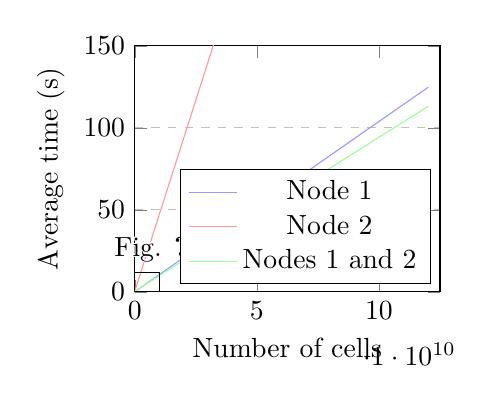
\begin{tikzpicture}
\begin{axis}[
    %title={Average time to compute edit distance},
    xlabel={Number of cells},
    ylabel={Average time (s)},
    xmin=0, xmax=125000000000,
    ymin=0, ymax=150,
    legend pos=south east,
    ymajorgrids=true,
    grid style=dashed,
    scaled x ticks={real:10000000000},
    width=0.45\linewidth,
]


\addplot[
    color=blue,
    smooth,
    ]
    coordinates {
    (16777216, 0.09921685714285713)(33554432, 0.12080128571428571)(67108864, 0.160687)(134217728, 0.2424785714285714)(268435456, 0.38340228571428575)(536870912, 0.6664877142857142)(1000000000, 1.152977142857143)(1500000000, 1.6785985714285712)(2147483648, 2.357917142857143)(3000000000, 3.2444357142857143)(4294967296, 4.582278571428572)(6000000000, 6.368568571428573)(7000000000, 7.4005728571428575)(8589934592, 9.062895000000001)(10000000000, 10.52197142857143)(11000000000, 11.564114285714284)(12000000000, 12.593114285714284)(13000000000, 13.643714285714285)(14000000000, 14.677214285714285)(17179869184, 17.97048571428571)(25769803776, 26.88624285714286)(34359738368, 35.8241)(42949672960, 44.70372857142858)(51539607552, 53.59438571428571)(60129542144, 62.536071428571425)(68719476736, 71.40738571428571)(77309411328, 80.32997142857143)(85899345920, 89.26152857142857)(94489280512, 98.17172857142855)(100000000000, 103.8337142857143)(103079215104, 107.02371428571429)(111669149696, 115.95128571428572)(120259084288, 124.80914285714286)
    };

\addplot[
    color=red,
    smooth,
    ]
    coordinates {
    (16777216, 0.5445155714285714)(33554432, 0.626533)(67108864, 0.8027252857142858)(134217728, 1.12474)(268435456, 1.7438942857142856)(536870912, 3.0209571428571427)(1000000000, 5.162437142857143)(1500000000, 7.543924285714286)(2147483648, 10.5999)(3000000000, 14.472014285714282)(4294967296, 20.55514285714286)(6000000000, 28.49077142857143)(7000000000, 33.10725714285714)(8589934592, 40.61537142857143)(10000000000, 47.16012857142857)(11000000000, 51.74827142857142)(12000000000, 56.35255714285715)(13000000000, 61.09289999999999)(14000000000, 65.73704285714287)(17179869184, 80.55284285714286)(25769803776, 120.55142857142857)(34359738368, 160.5607142857143)(42949672960, 200.45)(51539607552, 240.47842857142857)(60129542144, 280.283)(68719476736, 320.3165714285714)(77309411328, 360.40957142857144)(85899345920, 400.24628571428576)(94489280512, 440.2641428571429)(100000000000, 465.98900000000003)(103079215104, 480.2848571428571)(111669149696, 520.3457142857143)(120259084288, 560.304)
    };

\addplot[
    color=green,
    smooth,
    ]
    coordinates {
    (16777216, 0.496333)(33554432, 0.5080268571428571)(67108864, 0.6234567142857143)(134217728, 0.6975642857142856)(268435456, 0.7566615714285714)(536870912, 1.0175524285714288)(1000000000, 1.4202885714285713)(1500000000, 1.9164114285714287)(2147483648, 2.5176842857142856)(3000000000, 3.249014285714286)(4294967296, 4.516901428571428)(6000000000, 6.0832242857142855)(7000000000, 7.0254957142857135)(8589934592, 8.529228)(10000000000, 9.85383)(11000000000, 10.788914285714286)(12000000000, 11.679885714285714)(13000000000, 12.648942857142856)(14000000000, 13.559485714285714)(17179869184, 16.574385714285714)(25769803776, 24.604942857142856)(34359738368, 32.70814285714285)(42949672960, 40.747)(51539607552, 48.7744)(60129542144, 56.66547142857142)(68719476736, 64.66221428571428)(77309411328, 72.89688571428572)(85899345920, 81.01222857142857)(94489280512, 89.02959999999999)(100000000000, 94.25682857142858)(103079215104, 97.06402857142858)(111669149696, 105.15614285714285)(120259084288, 113.20742857142857)
    };

\addplot[
    color=black,
    mark=none,
] coordinates {(0,0) (0,12) (10000000000,12) (10000000000,0) (0,0)};

\pgfplotsset{
    after end axis/.code={
        \node[above] at (axis cs:10000000000,12){\contour{white}{Fig. \ref{result_graph_zoom}}};
    }
}


\legend{Node 1, Node 2, Nodes 1 and 2}
\end{axis}
\end{tikzpicture}

\end{frame}
\begin{frame}
    
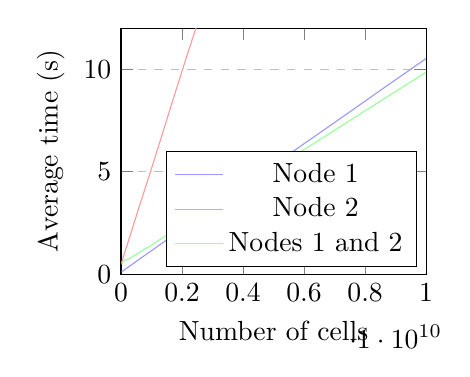
\begin{tikzpicture}
\begin{axis}[
    %title={Average time to compute edit distance},
    xlabel={Number of cells},
    ylabel={Average time (s)},
    xmin=0, xmax=10000000000,
    ymin=0, ymax=12,
    legend pos=south east,
    ymajorgrids=true,
    grid style=dashed,
    scaled x ticks={real:10000000000},
    width=0.45\linewidth,
]


\addplot[
    color=blue,
    smooth,
    ]
    coordinates {
    (16777216, 0.09921685714285713)(33554432, 0.12080128571428571)(67108864, 0.160687)(134217728, 0.2424785714285714)(268435456, 0.38340228571428575)(536870912, 0.6664877142857142)(1000000000, 1.152977142857143)(1500000000, 1.6785985714285712)(2147483648, 2.357917142857143)(3000000000, 3.2444357142857143)(4294967296, 4.582278571428572)(6000000000, 6.368568571428573)(7000000000, 7.4005728571428575)(8589934592, 9.062895000000001)(10000000000, 10.52197142857143)(11000000000, 11.564114285714284)(12000000000, 12.593114285714284)(13000000000, 13.643714285714285)(14000000000, 14.677214285714285)(17179869184, 17.97048571428571)(25769803776, 26.88624285714286)(34359738368, 35.8241)(42949672960, 44.70372857142858)(51539607552, 53.59438571428571)(60129542144, 62.536071428571425)(68719476736, 71.40738571428571)(77309411328, 80.32997142857143)(85899345920, 89.26152857142857)(94489280512, 98.17172857142855)(100000000000, 103.8337142857143)(103079215104, 107.02371428571429)(111669149696, 115.95128571428572)(120259084288, 124.80914285714286)
    };

\addplot[
    color=red,
    smooth,
    ]
    coordinates {
    (16777216, 0.5445155714285714)(33554432, 0.626533)(67108864, 0.8027252857142858)(134217728, 1.12474)(268435456, 1.7438942857142856)(536870912, 3.0209571428571427)(1000000000, 5.162437142857143)(1500000000, 7.543924285714286)(2147483648, 10.5999)(3000000000, 14.472014285714282)(4294967296, 20.55514285714286)(6000000000, 28.49077142857143)(7000000000, 33.10725714285714)(8589934592, 40.61537142857143)(10000000000, 47.16012857142857)(11000000000, 51.74827142857142)(12000000000, 56.35255714285715)(13000000000, 61.09289999999999)(14000000000, 65.73704285714287)(17179869184, 80.55284285714286)(25769803776, 120.55142857142857)(34359738368, 160.5607142857143)(42949672960, 200.45)(51539607552, 240.47842857142857)(60129542144, 280.283)(68719476736, 320.3165714285714)(77309411328, 360.40957142857144)(85899345920, 400.24628571428576)(94489280512, 440.2641428571429)(100000000000, 465.98900000000003)(103079215104, 480.2848571428571)(111669149696, 520.3457142857143)(120259084288, 560.304)
    };

\addplot[
    color=green,
    smooth,
    ]
    coordinates {
    (16777216, 0.496333)(33554432, 0.5080268571428571)(67108864, 0.6234567142857143)(134217728, 0.6975642857142856)(268435456, 0.7566615714285714)(536870912, 1.0175524285714288)(1000000000, 1.4202885714285713)(1500000000, 1.9164114285714287)(2147483648, 2.5176842857142856)(3000000000, 3.249014285714286)(4294967296, 4.516901428571428)(6000000000, 6.0832242857142855)(7000000000, 7.0254957142857135)(8589934592, 8.529228)(10000000000, 9.85383)(11000000000, 10.788914285714286)(12000000000, 11.679885714285714)(13000000000, 12.648942857142856)(14000000000, 13.559485714285714)(17179869184, 16.574385714285714)(25769803776, 24.604942857142856)(34359738368, 32.70814285714285)(42949672960, 40.747)(51539607552, 48.7744)(60129542144, 56.66547142857142)(68719476736, 64.66221428571428)(77309411328, 72.89688571428572)(85899345920, 81.01222857142857)(94489280512, 89.02959999999999)(100000000000, 94.25682857142858)(103079215104, 97.06402857142858)(111669149696, 105.15614285714285)(120259084288, 113.20742857142857)
    };


\legend{Node 1, Node 2, Nodes 1 and 2}
\end{axis}
\end{tikzpicture}

\end{frame}

\begin{frame}{Performance}
	Conclusion from test with $12\cdot10^{10}$ cells:
	\begin{itemize}
		\item Optimal theoretical performance: \\
			  $\frac{1}{ \frac{1}{124.81} + \frac{1}{560.30} }=102.1$ seconds
		\item Efficiency: \\
			  $\frac{102.07}{113.21}=90.16\%$
		\item Overhead: \\
			  $100\% - \frac{560.3/5}{113.2} \cdot 100\%=1.01\%$
		\item Solutions:
		\begin{itemize}
			\item Equivalent nodes
			\item Dynamic partitioning
		\end{itemize}
	\end{itemize}
\end{frame}

\begin{frame}{Conclusion}
Edit distance on GPU clusters using MPI
\end{frame}

\backupbegin
\setside{5}

\begin{frame}
	\includesvg[height=0.80\paperheight]{cols2}
	\hspace{1em}
	\includesvg[height=0.80\paperheight]{singlevar}
\end{frame}

\begin{frame}{More results}
	\begin{tabular}{r|r|r|r}
		Cells $\times10^{10}$ & Node 1 & Node 2 & Both nodes \\ \hline
		1.0 & 10.52 & 47.16 & 9.854 \\
		2.5 & 26.89 & 120.6 & 24.60 \\
		3.4 & 35.82 & 160.6 & 32.71 \\
		4.2 & 44.70 & 200.4 & 40.75 \\
		5.1 & 53.59 & 240.5 & 48.77 \\
		6.8 & 71.41 & 320.3 & 64.66 \\
		7.7 & 80.33 & 360.4 & 72.90 \\
		8.5 & 89.26 & 400.2 & 81.01 \\
		9.4 & 98.17 & 440.3 & 89.03 \\
		10.3 & 107.0 & 480.3 & 97.06 \\
		11.1 & 116.0 & 520.3 & 105.2 \\
		12.0 & 124.8 & 560.3 & 113.2 \\
	\end{tabular}
\end{frame}

\begin{frame}
    \begin{center}
\begin{tabular}{|c|c||c|c|c|c|c|c|c|c|}\hline
  &   & \textbf{S} & \textbf{a} & \textbf{t} & \textbf{u} & \textbf{r} & \textbf{d} & \textbf{a} & \textbf{y} \\\hline
  & 0 & 1 & 2 & 3 & 4 & 5 & 6 & 7 & 8 \\\hline\hline
\textbf{S} & 1 & 0 & 1 & 2 & 3 & 4 & 5 & 6 & 7 \\\hline
\textbf{u} & 2 & 1 & 1 & 2 & 2 & 3 & 4 & 5 & 6 \\\hline
\textbf{n} & 3 & 2 & 2 & 2 & 3 & 3 & 4 & 5 & 6 \\\hline
\textbf{d} & 4 & 3 & 3 & 3 & 3 & 4 & 3 & 4 & 5 \\\hline
\textbf{a} & 5 & 4 & 3 & 4 & 4 & 4 & 4 & 3 & 4 \\\hline
\textbf{y} & 6 & 5 & 4 & 4 & 5 & 5 & 5 & 4 & 3 \\\hline
    \end{tabular}
    \end{center}

\end{frame}


%\setbeamersize{text margin left=0.03\paperwidth,text margin right=0.03\paperwidth}
% \setbeamertemplate{background}{}
\begin{frame}
\small
% \begin{algorithm}
% \begin{multicols}{2}
\begin{algorithmic}[1]
\Procedure{Block\_calc}{$id, width, s_a, s_b, height, d$}
     \State{$a \gets s_a[width - 1 - id]$}\label{block:a}
    \For{$i$ is $0 \dots height$}\label{block:forbegin}
        \State{\Call{barrier}{\relax}} \label{block:barrier}
        \If{$a = s_b[id + i]$}\label{block:ifscorebegin}
            \State $Score \gets 0$
        \Else
            \State $Score \gets 1$
        \EndIf\label{block:ifscoreend}
        \State{$x \gets i + id \cdot 2 + 1$}\label{block:x}
        \State{$cell\_d \gets d[x] + Score$}\label{block:d}
        \State{$cell\_up \gets d[x - 1] + 1$}\label{block:up}
        \State{$\mathit{cell\_left} \gets d[x + 1] + 1$}\label{block:left}
        \State{$d[x] \gets $\Call{minimum}{$cell\_up, \mathit{cell\_left}, cell\_d$}}\label{block:write}
    \EndFor\label{block:forend}
\EndProcedure
\end{algorithmic}
% \end{multicols}
% \end{algorithm}

\end{frame}

\begin{frame}
    
\begin{tikzpicture}
\begin{axis}[
    %title={Average time to compute edit distance},
    xlabel={Number of cells},
    ylabel={Average time (s)},
    xmin=0, xmax=125000000000,
    ymin=0, ymax=600,
    legend pos=north west,
    ymajorgrids=true,
    grid style=dashed,
    scaled x ticks={real:10000000000},
    height=0.85\paperheight,
]


\addplot[
    color=blue,
    smooth,mark=\nodea
    ]
    coordinates {
    (16777216, 0.09921685714285713)(33554432, 0.12080128571428571)(67108864, 0.160687)(134217728, 0.2424785714285714)(268435456, 0.38340228571428575)(536870912, 0.6664877142857142)(1000000000, 1.152977142857143)(1500000000, 1.6785985714285712)(2147483648, 2.357917142857143)(3000000000, 3.2444357142857143)(4294967296, 4.582278571428572)(6000000000, 6.368568571428573)(7000000000, 7.4005728571428575)(8589934592, 9.062895000000001)(10000000000, 10.52197142857143)(11000000000, 11.564114285714284)(12000000000, 12.593114285714284)(13000000000, 13.643714285714285)(14000000000, 14.677214285714285)(17179869184, 17.97048571428571)(25769803776, 26.88624285714286)(34359738368, 35.8241)(42949672960, 44.70372857142858)(51539607552, 53.59438571428571)(60129542144, 62.536071428571425)(68719476736, 71.40738571428571)(77309411328, 80.32997142857143)(85899345920, 89.26152857142857)(94489280512, 98.17172857142855)(100000000000, 103.8337142857143)(103079215104, 107.02371428571429)(111669149696, 115.95128571428572)(120259084288, 124.80914285714286)
    };

\addplot[
    color=red,
    smooth,mark=\nodeb
    ]
    coordinates {
    (16777216, 0.5445155714285714)(33554432, 0.626533)(67108864, 0.8027252857142858)(134217728, 1.12474)(268435456, 1.7438942857142856)(536870912, 3.0209571428571427)(1000000000, 5.162437142857143)(1500000000, 7.543924285714286)(2147483648, 10.5999)(3000000000, 14.472014285714282)(4294967296, 20.55514285714286)(6000000000, 28.49077142857143)(7000000000, 33.10725714285714)(8589934592, 40.61537142857143)(10000000000, 47.16012857142857)(11000000000, 51.74827142857142)(12000000000, 56.35255714285715)(13000000000, 61.09289999999999)(14000000000, 65.73704285714287)(17179869184, 80.55284285714286)(25769803776, 120.55142857142857)(34359738368, 160.5607142857143)(42949672960, 200.45)(51539607552, 240.47842857142857)(60129542144, 280.283)(68719476736, 320.3165714285714)(77309411328, 360.40957142857144)(85899345920, 400.24628571428576)(94489280512, 440.2641428571429)(100000000000, 465.98900000000003)(103079215104, 480.2848571428571)(111669149696, 520.3457142857143)(120259084288, 560.304)
    };

\addplot[
    color=green,
    smooth,mark=\nodec
    ]
    coordinates {
    (16777216, 0.496333)(33554432, 0.5080268571428571)(67108864, 0.6234567142857143)(134217728, 0.6975642857142856)(268435456, 0.7566615714285714)(536870912, 1.0175524285714288)(1000000000, 1.4202885714285713)(1500000000, 1.9164114285714287)(2147483648, 2.5176842857142856)(3000000000, 3.249014285714286)(4294967296, 4.516901428571428)(6000000000, 6.0832242857142855)(7000000000, 7.0254957142857135)(8589934592, 8.529228)(10000000000, 9.85383)(11000000000, 10.788914285714286)(12000000000, 11.679885714285714)(13000000000, 12.648942857142856)(14000000000, 13.559485714285714)(17179869184, 16.574385714285714)(25769803776, 24.604942857142856)(34359738368, 32.70814285714285)(42949672960, 40.747)(51539607552, 48.7744)(60129542144, 56.66547142857142)(68719476736, 64.66221428571428)(77309411328, 72.89688571428572)(85899345920, 81.01222857142857)(94489280512, 89.02959999999999)(100000000000, 94.25682857142858)(103079215104, 97.06402857142858)(111669149696, 105.15614285714285)(120259084288, 113.20742857142857)
    };

\addplot[
    color=black,
    mark=none,
] coordinates {(0,0) (0,12) (10000000000,12) (10000000000,0) (0,0)};

\pgfplotsset{
    after end axis/.code={
        \node[above] at (axis cs:10000000000,12){\contour{white}{Zoom}};
    }
}


\legend{Node 1, Node 2, Nodes 1 and 2}
\end{axis}
\end{tikzpicture}

\end{frame}

\renewcommand\nodea[0]{diamond}
\renewcommand\nodeb[0]{triangle}
\renewcommand\nodec[0]{square}

\begin{frame}
    
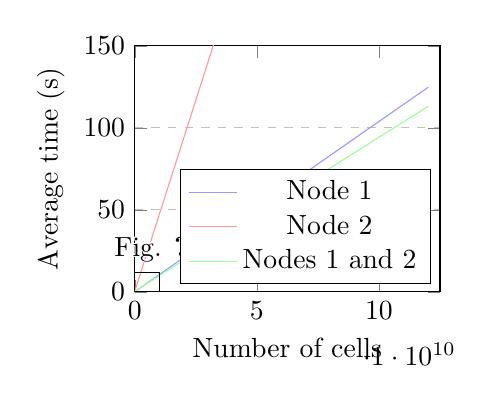
\begin{tikzpicture}
\begin{axis}[
    %title={Average time to compute edit distance},
    xlabel={Number of cells},
    ylabel={Average time (s)},
    xmin=0, xmax=125000000000,
    ymin=0, ymax=150,
    legend pos=south east,
    ymajorgrids=true,
    grid style=dashed,
    scaled x ticks={real:10000000000},
    width=0.45\linewidth,
]


\addplot[
    color=blue,
    smooth,
    ]
    coordinates {
    (16777216, 0.09921685714285713)(33554432, 0.12080128571428571)(67108864, 0.160687)(134217728, 0.2424785714285714)(268435456, 0.38340228571428575)(536870912, 0.6664877142857142)(1000000000, 1.152977142857143)(1500000000, 1.6785985714285712)(2147483648, 2.357917142857143)(3000000000, 3.2444357142857143)(4294967296, 4.582278571428572)(6000000000, 6.368568571428573)(7000000000, 7.4005728571428575)(8589934592, 9.062895000000001)(10000000000, 10.52197142857143)(11000000000, 11.564114285714284)(12000000000, 12.593114285714284)(13000000000, 13.643714285714285)(14000000000, 14.677214285714285)(17179869184, 17.97048571428571)(25769803776, 26.88624285714286)(34359738368, 35.8241)(42949672960, 44.70372857142858)(51539607552, 53.59438571428571)(60129542144, 62.536071428571425)(68719476736, 71.40738571428571)(77309411328, 80.32997142857143)(85899345920, 89.26152857142857)(94489280512, 98.17172857142855)(100000000000, 103.8337142857143)(103079215104, 107.02371428571429)(111669149696, 115.95128571428572)(120259084288, 124.80914285714286)
    };

\addplot[
    color=red,
    smooth,
    ]
    coordinates {
    (16777216, 0.5445155714285714)(33554432, 0.626533)(67108864, 0.8027252857142858)(134217728, 1.12474)(268435456, 1.7438942857142856)(536870912, 3.0209571428571427)(1000000000, 5.162437142857143)(1500000000, 7.543924285714286)(2147483648, 10.5999)(3000000000, 14.472014285714282)(4294967296, 20.55514285714286)(6000000000, 28.49077142857143)(7000000000, 33.10725714285714)(8589934592, 40.61537142857143)(10000000000, 47.16012857142857)(11000000000, 51.74827142857142)(12000000000, 56.35255714285715)(13000000000, 61.09289999999999)(14000000000, 65.73704285714287)(17179869184, 80.55284285714286)(25769803776, 120.55142857142857)(34359738368, 160.5607142857143)(42949672960, 200.45)(51539607552, 240.47842857142857)(60129542144, 280.283)(68719476736, 320.3165714285714)(77309411328, 360.40957142857144)(85899345920, 400.24628571428576)(94489280512, 440.2641428571429)(100000000000, 465.98900000000003)(103079215104, 480.2848571428571)(111669149696, 520.3457142857143)(120259084288, 560.304)
    };

\addplot[
    color=green,
    smooth,
    ]
    coordinates {
    (16777216, 0.496333)(33554432, 0.5080268571428571)(67108864, 0.6234567142857143)(134217728, 0.6975642857142856)(268435456, 0.7566615714285714)(536870912, 1.0175524285714288)(1000000000, 1.4202885714285713)(1500000000, 1.9164114285714287)(2147483648, 2.5176842857142856)(3000000000, 3.249014285714286)(4294967296, 4.516901428571428)(6000000000, 6.0832242857142855)(7000000000, 7.0254957142857135)(8589934592, 8.529228)(10000000000, 9.85383)(11000000000, 10.788914285714286)(12000000000, 11.679885714285714)(13000000000, 12.648942857142856)(14000000000, 13.559485714285714)(17179869184, 16.574385714285714)(25769803776, 24.604942857142856)(34359738368, 32.70814285714285)(42949672960, 40.747)(51539607552, 48.7744)(60129542144, 56.66547142857142)(68719476736, 64.66221428571428)(77309411328, 72.89688571428572)(85899345920, 81.01222857142857)(94489280512, 89.02959999999999)(100000000000, 94.25682857142858)(103079215104, 97.06402857142858)(111669149696, 105.15614285714285)(120259084288, 113.20742857142857)
    };

\addplot[
    color=black,
    mark=none,
] coordinates {(0,0) (0,12) (10000000000,12) (10000000000,0) (0,0)};

\pgfplotsset{
    after end axis/.code={
        \node[above] at (axis cs:10000000000,12){\contour{white}{Fig. \ref{result_graph_zoom}}};
    }
}


\legend{Node 1, Node 2, Nodes 1 and 2}
\end{axis}
\end{tikzpicture}

\end{frame}
\begin{frame}
    
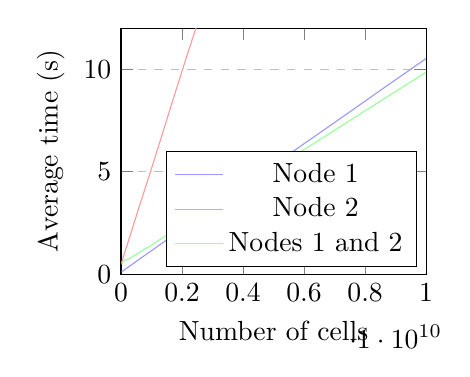
\begin{tikzpicture}
\begin{axis}[
    %title={Average time to compute edit distance},
    xlabel={Number of cells},
    ylabel={Average time (s)},
    xmin=0, xmax=10000000000,
    ymin=0, ymax=12,
    legend pos=south east,
    ymajorgrids=true,
    grid style=dashed,
    scaled x ticks={real:10000000000},
    width=0.45\linewidth,
]


\addplot[
    color=blue,
    smooth,
    ]
    coordinates {
    (16777216, 0.09921685714285713)(33554432, 0.12080128571428571)(67108864, 0.160687)(134217728, 0.2424785714285714)(268435456, 0.38340228571428575)(536870912, 0.6664877142857142)(1000000000, 1.152977142857143)(1500000000, 1.6785985714285712)(2147483648, 2.357917142857143)(3000000000, 3.2444357142857143)(4294967296, 4.582278571428572)(6000000000, 6.368568571428573)(7000000000, 7.4005728571428575)(8589934592, 9.062895000000001)(10000000000, 10.52197142857143)(11000000000, 11.564114285714284)(12000000000, 12.593114285714284)(13000000000, 13.643714285714285)(14000000000, 14.677214285714285)(17179869184, 17.97048571428571)(25769803776, 26.88624285714286)(34359738368, 35.8241)(42949672960, 44.70372857142858)(51539607552, 53.59438571428571)(60129542144, 62.536071428571425)(68719476736, 71.40738571428571)(77309411328, 80.32997142857143)(85899345920, 89.26152857142857)(94489280512, 98.17172857142855)(100000000000, 103.8337142857143)(103079215104, 107.02371428571429)(111669149696, 115.95128571428572)(120259084288, 124.80914285714286)
    };

\addplot[
    color=red,
    smooth,
    ]
    coordinates {
    (16777216, 0.5445155714285714)(33554432, 0.626533)(67108864, 0.8027252857142858)(134217728, 1.12474)(268435456, 1.7438942857142856)(536870912, 3.0209571428571427)(1000000000, 5.162437142857143)(1500000000, 7.543924285714286)(2147483648, 10.5999)(3000000000, 14.472014285714282)(4294967296, 20.55514285714286)(6000000000, 28.49077142857143)(7000000000, 33.10725714285714)(8589934592, 40.61537142857143)(10000000000, 47.16012857142857)(11000000000, 51.74827142857142)(12000000000, 56.35255714285715)(13000000000, 61.09289999999999)(14000000000, 65.73704285714287)(17179869184, 80.55284285714286)(25769803776, 120.55142857142857)(34359738368, 160.5607142857143)(42949672960, 200.45)(51539607552, 240.47842857142857)(60129542144, 280.283)(68719476736, 320.3165714285714)(77309411328, 360.40957142857144)(85899345920, 400.24628571428576)(94489280512, 440.2641428571429)(100000000000, 465.98900000000003)(103079215104, 480.2848571428571)(111669149696, 520.3457142857143)(120259084288, 560.304)
    };

\addplot[
    color=green,
    smooth,
    ]
    coordinates {
    (16777216, 0.496333)(33554432, 0.5080268571428571)(67108864, 0.6234567142857143)(134217728, 0.6975642857142856)(268435456, 0.7566615714285714)(536870912, 1.0175524285714288)(1000000000, 1.4202885714285713)(1500000000, 1.9164114285714287)(2147483648, 2.5176842857142856)(3000000000, 3.249014285714286)(4294967296, 4.516901428571428)(6000000000, 6.0832242857142855)(7000000000, 7.0254957142857135)(8589934592, 8.529228)(10000000000, 9.85383)(11000000000, 10.788914285714286)(12000000000, 11.679885714285714)(13000000000, 12.648942857142856)(14000000000, 13.559485714285714)(17179869184, 16.574385714285714)(25769803776, 24.604942857142856)(34359738368, 32.70814285714285)(42949672960, 40.747)(51539607552, 48.7744)(60129542144, 56.66547142857142)(68719476736, 64.66221428571428)(77309411328, 72.89688571428572)(85899345920, 81.01222857142857)(94489280512, 89.02959999999999)(100000000000, 94.25682857142858)(103079215104, 97.06402857142858)(111669149696, 105.15614285714285)(120259084288, 113.20742857142857)
    };


\legend{Node 1, Node 2, Nodes 1 and 2}
\end{axis}
\end{tikzpicture}

\end{frame}
\begin{frame}
    
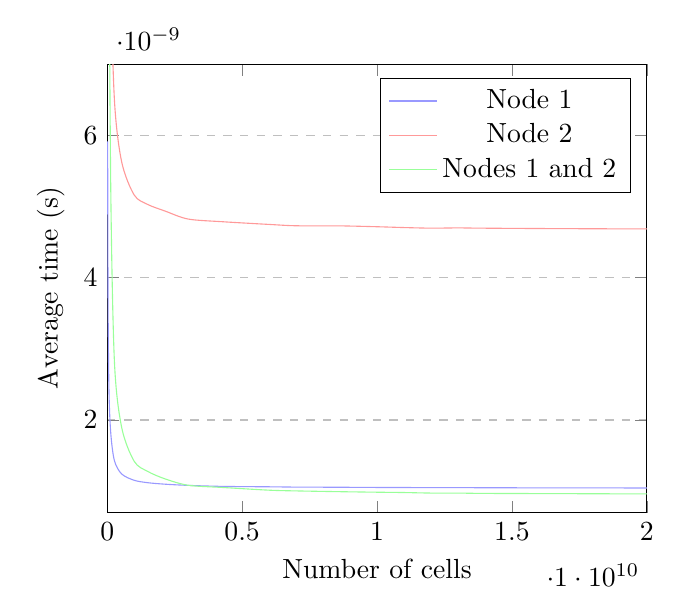
\begin{tikzpicture}
\begin{axis}[
    %title={Average time per cell},
    xlabel={Number of cells},
    ylabel={Average time (s)},
    xmin=0, xmax=20000000000,
    ymin=7e-10, ymax=7e-09,
    legend pos=north east,
    ymajorgrids=true,
    grid style=dashed,
    scaled x ticks={real:10000000000},
]


\addplot[
    color=blue,
    smooth,
    ]
    coordinates {
    (16777216, 5.9137855257306775e-09)(33554432, 3.600158861705235e-09)(67108864, 2.3944228887557983e-09)(134217728, 1.8066061394555226e-09)(268435456, 1.4282848153795516e-09)(536870912, 1.2414301080363135e-09)(1000000000, 1.152977142857143e-09)(1500000000, 1.119065714285714e-09)(2147483648, 1.0979907321078438e-09)(3000000000, 1.0814785714285714e-09)(4294967296, 1.0668948691870486e-09)(6000000000, 1.0614280952380955e-09)(7000000000, 1.057224693877551e-09)(8589934592, 1.0550598381087185e-09)(10000000000, 1.0521971428571429e-09)(11000000000, 1.0512831168831168e-09)(12000000000, 1.0494261904761902e-09)(13000000000, 1.0495164835164835e-09)(14000000000, 1.0483724489795918e-09)(17179869184, 1.0460199389074528e-09)(25769803776, 1.0433235383104711e-09)(34359738368, 1.042618532665074e-09)(42949672960, 1.0408397897013597e-09)(51539607552, 1.0398679435075748e-09)(60129542144, 1.0400224115927607e-09)(68719476736, 1.0391142235935798e-09)(77309411328, 1.0390710529117357e-09)(85899345920, 1.0391409575406993e-09)(94489280512, 1.0389721250863041e-09)(100000000000, 1.0383371428571429e-09)(103079215104, 1.0382666784737793e-09)(111669149696, 1.038346634051957e-09)(120259084288, 1.0378354666184407e-09)
    };

\addplot[
    color=red,
    smooth,
    ]
    coordinates {
    (16777216, 3.245565720966884e-08)(33554432, 1.8672138452529907e-08)(67108864, 1.1961538876805988e-08)(134217728, 8.379966020584107e-09)(268435456, 6.4965124641145975e-09)(536870912, 5.626971168177468e-09)(1000000000, 5.162437142857143e-09)(1500000000, 5.029282857142857e-09)(2147483648, 4.935963079333305e-09)(3000000000, 4.824004761904761e-09)(4294967296, 4.785867141825813e-09)(6000000000, 4.748461904761905e-09)(7000000000, 4.729608163265305e-09)(8589934592, 4.728251535977636e-09)(10000000000, 4.7160128571428574e-09)(11000000000, 4.704388311688311e-09)(12000000000, 4.696046428571429e-09)(13000000000, 4.699453846153845e-09)(14000000000, 4.695503061224491e-09)(17179869184, 4.688792562644397e-09)(25769803776, 4.678011117946534e-09)(34359738368, 4.6729318065834904e-09)(42949672960, 4.667090252041816e-09)(51539607552, 4.665895609096402e-09)(60129542144, 4.661319378231253e-09)(68719476736, 4.661219593669687e-09)(77309411328, 4.661910694151644e-09)(85899345920, 4.659480016146388e-09)(94489280512, 4.6594083526885355e-09)(100000000000, 4.6598900000000005e-09)(103079215104, 4.659376351074094e-09)(111669149696, 4.6597087530644385e-09)(120259084288, 4.659140748637063e-09)
    };

\addplot[
    color=green,
    smooth,
    ]
    coordinates {
    (16777216, 2.9583752155303957e-08)(33554432, 1.514038017817906e-08)(67108864, 9.290228996958051e-09)(134217728, 5.197258932249886e-09)(268435456, 2.8187840112618036e-09)(536870912, 1.8953390951667517e-09)(1000000000, 1.4202885714285714e-09)(1500000000, 1.277607619047619e-09)(2147483648, 1.1723881055201802e-09)(3000000000, 1.083004761904762e-09)(4294967296, 1.0516730669353688e-09)(6000000000, 1.0138707142857144e-09)(7000000000, 1.003642244897959e-09)(8589934592, 9.929328225553036e-10)(10000000000, 9.85383e-10)(11000000000, 9.808103896103896e-10)(12000000000, 9.733238095238094e-10)(13000000000, 9.729956043956044e-10)(14000000000, 9.68534693877551e-10)(17179869184, 9.647562235061612e-10)(25769803776, 9.547974470825421e-10)(34359738368, 9.519322442689111e-10)(42949672960, 9.487150236964226e-10)(51539607552, 9.463479121526082e-10)(60129542144, 9.423898704045889e-10)(68719476736, 9.409590607642063e-10)(77309411328, 9.429238234010953e-10)(85899345920, 9.43106466106006e-10)(94489280512, 9.422190487384794e-10)(100000000000, 9.425682857142859e-10)(103079215104, 9.416450103301378e-10)(111669149696, 9.416758625225706e-10)(120259084288, 9.41362802167328e-10)
    };


\legend{Node 1, Node 2, Nodes 1 and 2}
\end{axis}
\end{tikzpicture}

\end{frame}
\begin{frame}
    
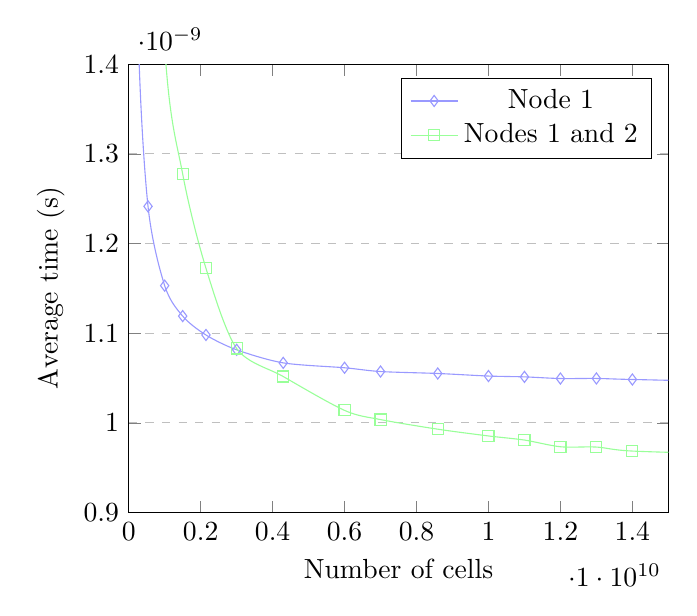
\begin{tikzpicture}
\begin{axis}[
    %title={Average time per cell},
    xlabel={Number of cells},
    ylabel={Average time (s)},
    xmin=0, xmax=15000000000,
    ymin=9e-10, ymax=1.4e-09,
    legend pos=north east,
    ymajorgrids=true,
    grid style=dashed,
    scaled x ticks={real:10000000000},
]


\addplot[
    color=blue,
    smooth,mark=diamond,
    ]
    coordinates {
    (16777216, 5.9137855257306775e-09)(33554432, 3.600158861705235e-09)(67108864, 2.3944228887557983e-09)(134217728, 1.8066061394555226e-09)(268435456, 1.4282848153795516e-09)(536870912, 1.2414301080363135e-09)(1000000000, 1.152977142857143e-09)(1500000000, 1.119065714285714e-09)(2147483648, 1.0979907321078438e-09)(3000000000, 1.0814785714285714e-09)(4294967296, 1.0668948691870486e-09)(6000000000, 1.0614280952380955e-09)(7000000000, 1.057224693877551e-09)(8589934592, 1.0550598381087185e-09)(10000000000, 1.0521971428571429e-09)(11000000000, 1.0512831168831168e-09)(12000000000, 1.0494261904761902e-09)(13000000000, 1.0495164835164835e-09)(14000000000, 1.0483724489795918e-09)(17179869184, 1.0460199389074528e-09)(25769803776, 1.0433235383104711e-09)(34359738368, 1.042618532665074e-09)(42949672960, 1.0408397897013597e-09)(51539607552, 1.0398679435075748e-09)(60129542144, 1.0400224115927607e-09)(68719476736, 1.0391142235935798e-09)(77309411328, 1.0390710529117357e-09)(85899345920, 1.0391409575406993e-09)(94489280512, 1.0389721250863041e-09)(100000000000, 1.0383371428571429e-09)(103079215104, 1.0382666784737793e-09)(111669149696, 1.038346634051957e-09)(120259084288, 1.0378354666184407e-09)
    };

\addplot[
    color=green,
    smooth,mark=square,
    ]
    coordinates {
    (16777216, 2.9583752155303957e-08)(33554432, 1.514038017817906e-08)(67108864, 9.290228996958051e-09)(134217728, 5.197258932249886e-09)(268435456, 2.8187840112618036e-09)(536870912, 1.8953390951667517e-09)(1000000000, 1.4202885714285714e-09)(1500000000, 1.277607619047619e-09)(2147483648, 1.1723881055201802e-09)(3000000000, 1.083004761904762e-09)(4294967296, 1.0516730669353688e-09)(6000000000, 1.0138707142857144e-09)(7000000000, 1.003642244897959e-09)(8589934592, 9.929328225553036e-10)(10000000000, 9.85383e-10)(11000000000, 9.808103896103896e-10)(12000000000, 9.733238095238094e-10)(13000000000, 9.729956043956044e-10)(14000000000, 9.68534693877551e-10)(17179869184, 9.647562235061612e-10)(25769803776, 9.547974470825421e-10)(34359738368, 9.519322442689111e-10)(42949672960, 9.487150236964226e-10)(51539607552, 9.463479121526082e-10)(60129542144, 9.423898704045889e-10)(68719476736, 9.409590607642063e-10)(77309411328, 9.429238234010953e-10)(85899345920, 9.43106466106006e-10)(94489280512, 9.422190487384794e-10)(100000000000, 9.425682857142859e-10)(103079215104, 9.416450103301378e-10)(111669149696, 9.416758625225706e-10)(120259084288, 9.41362802167328e-10)
    };


\legend{Node 1, Nodes 1 and 2}
\end{axis}
\end{tikzpicture}

\end{frame}

\backupend

\end{document}
